\documentclass[11pt,a4paper]{article}

% PAQUETES
\usepackage[T1]{fontenc}%
\usepackage[utf8]{inputenc}%

\usepackage[english]{babel}
\usepackage{amsmath}
\usepackage{amsthm}
\usepackage{amsfonts}
\usepackage[%left=1.54cm,right=1.54cm,top=1.54cm,bottom=1.54cm
    margin=1in,
]{geometry}
\usepackage{xfrac}  
\usepackage{tikz-cd}
\usepackage{enumerate}
\usepackage{amsfonts}
\usepackage{amssymb}
\usepackage{tcolorbox}
\usepackage{rotating}
\usepackage{mathpazo}
% \usepackage{charter}
\usetikzlibrary{babel}
\usepackage{listings}
\usepackage{amssymb}
\usepackage{extarrows}
\usepackage{makeidx}
\usepackage{graphicx}
\usepackage{multirow}
\usepackage{tikz-cd}
\usepackage{tasks}
\usepackage{xcolor}

% Christian
\usepackage{enumitem,etoolbox,titlesec}


%OPERADORES

\DeclareMathOperator{\dom}{dom}
\DeclareMathOperator{\cod}{cod}
\DeclareMathOperator{\id}{id}

\newcommand{\red}[1]{\textcolor{red}{#1}}
\newcommand{\C}{\mathbb{C}}
\newcommand{\im}{\text{Im}}
\newcommand{\R}{\mathbb{R}}
\newcommand{\N}{\mathbb{N}}
\newcommand{\Z}{\mathbb{Z}}
\newcommand{\D}{\mathbb{D}}
\newcommand{\B}{\mbox{Ob}}
\newcommand{\M}{\mbox{Mo}}
\newcommand{\del}{\Delta}
\newcommand{\odel}[1]{\left[#1\right]}
\newcommand{\Hom}[1]{\text{Hom}(#1)}
\newcommand{\adel}[1]{\left\lbrace #1 \right\rbrace}
%\renewcommand{\theequation}{\thesection.\arabic{equation}}
\newcommand{\funcion}[5]{%
{\setlength{\arraycolsep}{2pt}
\begin{array}{r@{}ccl}
#1\colon \hspace{0pt}& #2 & \longrightarrow & #3\\
& #4 & \longmapsto & #5
\end{array}}}

\newcommand{\func}[3]{#1\colon  #2  \to  #3}

\newcommand\restr[2]{{% we make the whole thing an ordinary symbol
  \left.\kern-\nulldelimiterspace % automatically resize the bar with \right
  #1 % the function
  \vphantom{\big|} % pretend it's a little taller at normal size
  \right|_{#2} % this is the delimiter
  }}

%ENTORNOS

% \theoremstyle{theorem}
\newtheorem{teo}{Theorem}[section]
\newtheorem{prop}[teo]{Proposition}
\newtheorem{lem}[teo]{Lemma}
\newtheorem{cor}[teo]{Corollary}

\theoremstyle{definition}
\newtheorem{defi}[teo]{Definition}
\newtheorem{rem}{Remark}[teo]
\newtheorem{exa}{Example}
\newtheorem{eje}{Exercise}
\newtheorem{que}{Question}

\newenvironment{sol}
  {\begin{proof}[\textit{Solution}]}
  {\end{proof}}

\titlelabel{\thetitle.\quad}

\def\contador{}
\graphicspath{{./figures/}}
\newcommand{\qand}{\quad\text{and}\quad}
\usepackage{microtype,parskip}
\setlength{\parindent}{15pt}
\linespread{1.15}
\usepackage{hyperref}
\hypersetup{
    colorlinks=true,  
    allcolors=blue,
    pdfproducer={Christian Chávez},
}

\makeatletter
\@ifclassloaded{exam}{
    \footer{}{\thepage}{}
    \renewcommand{\thequestion}{\bfseries\arabic{question}}
    \renewcommand{\solutiontitle}{\noindent\textit{Solution.}\enspace}
    \unframedsolutions
}{}
\makeatother


\newenvironment{theproof}
{
    \renewcommand{\solutiontitle}{}
    \begin{solution}
    \vspace*{-\baselineskip}
    \begin{proof}
}
{
    \end{proof}
    \end{solution}
    \renewcommand{\solutiontitle}{\noindent\textit{Solution.} }
}

\begin{document}

\def\contador{Lesson 4}
\noindent
\begin{minipage}[c]{0.33\textwidth}
    
\includegraphics[scale=0.37]{sello_yachay.png}
\end{minipage}
\begin{minipage}[c]{0.37\textwidth}
    % \centering
    \textbf{\large School of Mathematical and\\ Computational Sciences}\par
    Abstract Algebra
\end{minipage}
~ 
\begin{minipage}[c]{3mm}
    \raggedleft
    \rule[1.5mm]{0.3mm}{15mm}
\end{minipage}
~ 
\begin{minipage}[c]{0.24\textwidth}
    \raggedleft
    Prof. Pablo Rosero\\
    \& Christian Chávez\\
    \contador{}
\end{minipage}

\vspace{1mm}
\noindent\hrulefill

\vspace{3mm}

\section{The dihedral group}

Objects have bilateral
symmetry if they look the same when flipped over (usually in a specific direction, say vertically).
The easiest geometric examples of objects
with both rotational and bilateral symmetry are regular polygons.

\begin{figure}[!htb]
    \centering
    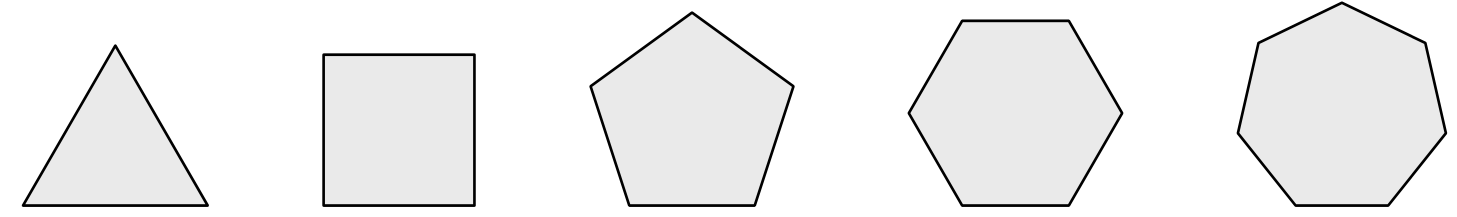
\includegraphics[width=0.75\textwidth]{polygons.png}
    % \caption{}%\label{fig:}
\end{figure}

Observe that is not necessary to track the movement of all the points that make up a  polygon in order to describe a rigid motion. 
Instead, we can simply keep track of their vertices.
This motivates  an important example of groups.

Some definitions first.
A permutation of a set \(X\) is a bijection from \(X\) onto \(X\).
A regular polygon with $n$ sides is called an $n$-gon.
A symmetry of the \(n\)-gon is any rigid motion of of the \(n\)-gon.
To be precise,  a symmetry of the \(n\)-gon is just a permutation of \(\left\{ 1,\ldots, n \right\}\). From now and on, we will denote \([n] = \left\{ 1,\ldots, n \right\}\).

It turns out, we can associate a group to the \(n\)-gon to study its rigid motions, that is, its symmetries.
It is called the dihedral group of order \(2n\) and denoted \(D_{2n}\).
Dihedral groups describe objects that have both rotational and bilateral symmetry.
Before defining precisely \(D_{2n}\), let us see an example.

% For example, 

\begin{exa}
    Both rotations and horizontal flips respect the shape of an equilateral triangle.

\begin{figure}[!htb]
    \centering
    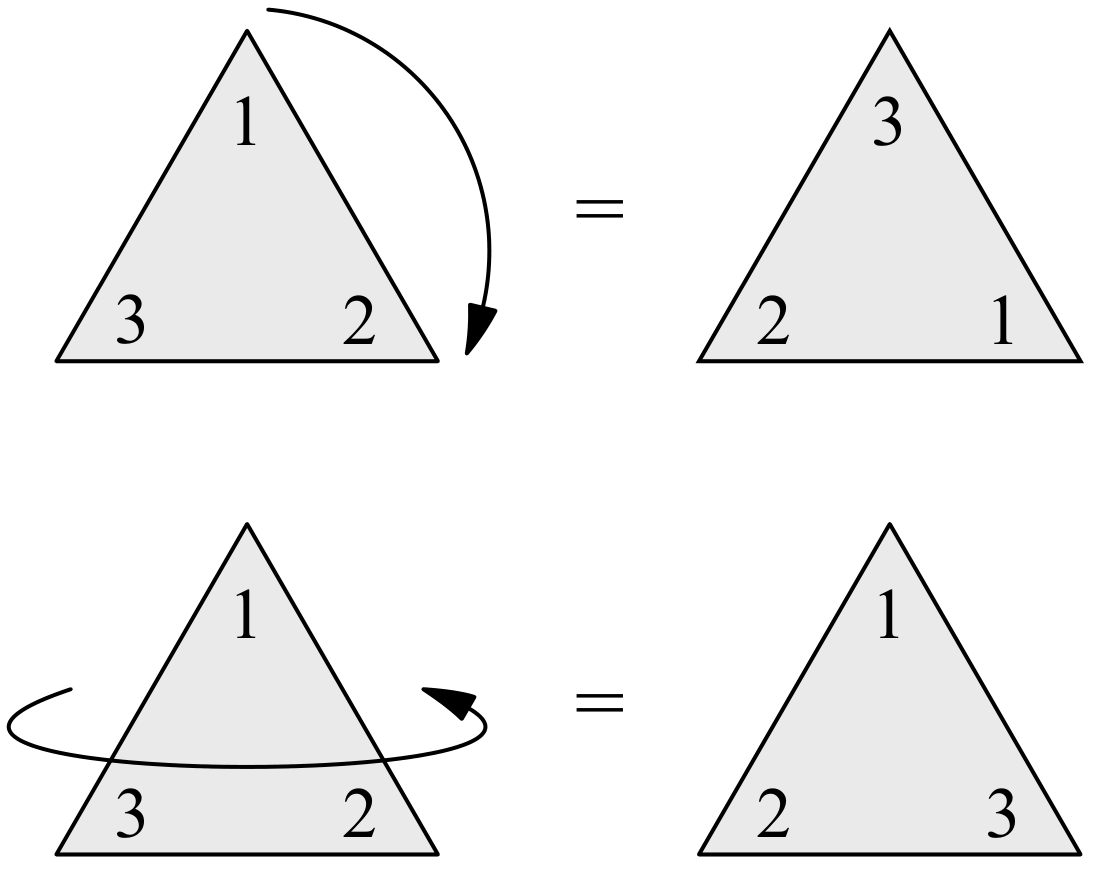
\includegraphics[width=0.3\textwidth]{triangle-rotation.png}
    % \caption{}%\label{fig:}
\end{figure}

The first symmetry is described by the permutation \(\sigma\colon [3]\to [3]\) defined by 
\[\sigma(1)=2,\quad\sigma(2)=3,\quad \sigma(3) = 1.\]

The second one is described by \(\tau\colon [3]\to [3]\) where 
\[\tau(1)=1,\quad\tau(2)=3,\quad \tau(3) = 2.\]
\end{exa}

Suppose we have  a regular \(n\)-gon centered at the origin in the plane and label the vertices consecutively from 1 to \(1\), clockwise.
\begin{enumerate}[label=(\roman*)]
    \item Let \(r\) be the rotation clockwise about the origin through \(2\pi / n\) radians. 
    \item  Let $s$ be the reflection about the line of symmetry through vertex 1 and the origin.
\end{enumerate}

The dihedral group \(D_{2n}\) is the set of rotations and reflections of the \(n\)-gon endowed with the following operation.
\begin{enumerate}[label=(\roman*),start=3]
    \item If \(a,b\in D_{2n}\), then \(ab\) is the symmetry obtained by first applying \(b\) and then \(a\) to the \(n\)-gon. 
\end{enumerate}





\begin{rem}
    \begin{itemize}
        % \item 
        \item We choose the notation \(D_{2n}\) because there are \(2n\) symmetries associated to a \(n\)-gon. Namely, \(n\) rotations and \(n\) reflections.
        \item The identity of \(D_{2n}\) is the identity symmetry, that is the effect of doing nothing to the \(n\)-gon.
        \item Think of the operation as function composition: we apply one function after another, writing the last application consecutively to the left.
    \end{itemize}
    
    
\end{rem}


\begin{teo}\hfill\null
\begin{enumerate}[label=(\roman*)]
    \item \(\left\{ 1,r,r^2,\ldots,r^{n-1} \right\}\) are all distinct,   \(r^n = 1\) and \(|r| = n\).
    \item \(|s| =2\)
    \item \(s\neq r^i\) for all \(i\in [n]_0\).
    \item \(sr^i = sr^j \) for all \(i,j\in [n-1]\) distinct.
    \item \(rs = sr^{-1}\), so \(D_{2n}\) is nonabelian
    \item \(r^i s = sr^{-i}\) for all \(0\leq i\leq n\)
\end{enumerate}
\end{teo}

\begin{proof}
    Classwork.
\end{proof}

\begin{rem}
    Facts \((i)\), \((ii)\) and \((v)\) are so important that they together serve to give an alternative definition of the dihedral group of order \(2n\), namely 
    \[D_{2 n}=\left\langle r, s \, \bigg|\,  r^n=s^2=1, r s=s r^{-1}\right\rangle.\]
\end{rem}

\begin{eje}
    Prove or disprove \((sr^9) (sr^6) = r^9\).
\end{eje}


\section{Permutations and the symmetric group}

Recall a permutation of a set \(X\) is a bijective function \(\alpha\colon X\to X\).
The set of all permutations of \(X \) is denoted \(S_X\).
If \(X\) is a finite set with \(n\) elements, then we choose the notation \( S_n\) instead and regard \(S_n\) as the set of bijections from \([n]\) to \([n]\).
The set \(S_X\) is a group under the operation of  composition of functions (why?).
We call \((S_X,\circ )\) the symmetric group on  \(X\).


There is a convenient way to denote the elements of \(S_n\). Keep in mind that an element \(\sigma\) of \(S_n\) is an injective function onto \([n]\) that is entirely determined by its values \(\sigma(1), \ldots,\sigma(n)\).
Let \(\sigma\in S_n\) be the permutation defined by 
\[\begin{tikzcd}
1 \arrow[rd, maps to]                      & 1 \\
2 \arrow[rdd, maps to] \arrow[ru, maps to] & 2 \\
3 \arrow[r, maps to]                       & 3 \\
4 \arrow[rd, maps to]                      & 4 \\
5 \arrow[ru, maps to]                      & 5
\end{tikzcd}\]

We come up with a useful notation: write   \((1\, 2)(3)(4\, 5)\) to represent \(\sigma\). This notation entirely captures what \(\sigma\) does to the set \([5]\). For instance, \((1\, 2)\) means \(\sigma\colon 1 \mapsto 2\) and \(\sigma\colon 2\mapsto 1\). Since \((3)\) means \(\sigma\colon 3 \mapsto 3\), that is, \(\sigma\) leaves \(3\) fixed, we can omit it from our notation and just  write  \((1\, 2)(4\, 5)\).

Let us formalize what we have seen.


A cycle is a string of integers which represents the element of $S_n$ which cyclically permutes these integers (and fixes all other integers). The cycle  $(a_1\,  a_2 \, \cdots\,  a_m)$  is the permutation which sends $a_i$ to $a_{i+1}$, for all $1 \leq i \leq m-1$ and sends $a_m$ to $a_1$ (so the cycle is closed). 

There is not a single way to write a cycle.
For instance, both 
\[(1\, 5\, 3\, 4\, 2)\quad\text{and}\quad (3\, 4\, 2\, 1\, 5)\]
denote the same permutation.

\begin{rem}
    It is also possible to use the   notation 
    \[\sigma ={\begin{pmatrix}{1}&{2}&{3}&\cdots &{n}\\\sigma ({1})&\sigma ( {2})&\sigma ({3})&\cdots &\sigma ({n})\end{pmatrix}}\]
    where the elements of \([n]\) are listed in the first row and their image  under \(\sigma\) below it in the second row.
    In this case, the order of the elements in the first row does not matter.
\end{rem}



\begin{lem}
    \(S_X\) is a nonabelian group.
\end{lem}

\begin{proof}
    In \(S_3\), take \(\sigma = (1\, 2\, 3 )\) and \(\tau = (1\, 2)\).
    We have 
    \[\sigma \circ \tau = (1\, 3)\quad\text{and}\quad \tau\circ \sigma = (2\, 3),\]
    which are not equal.
\end{proof}


\begin{defi}
    Let $i_1, i_2, \dots, i_r$ be distinct integers in $[n]$. If $\alpha \in S_n$ fixes the other integers (if any) and if
\[
\alpha(i_1) = i_2, \quad \alpha(i_2) = i_3, \quad \dots, \quad \alpha(i_{r-1}) = i_r, \quad \alpha(i_r) = i_1,
\]
then $\alpha$ is called an $r$-cycle.
\end{defi}

Given  \(\sigma\in S_X\), we say \(\sigma\) fixes \(x\in X\) if \(\sigma(x) = x\), otherwise \(\sigma\) moves \(x\).

A \(2\)-cycle is called a transposition.
A transposition interchanges two integers and fixes everything else.
Note that any \(1\)-cycle is the identity.

\paragraph*{Algorithm to factor a permutation into the product of cycles} 
\begin{itemize}
    \item To start a new cycle, pick the smallest element of $\{1, 2, \dots, n\}$ that has not yet appeared in a previous cycle. Call it $a$. If you are just starting, set $a = 1$. Begin the new cycle: $(a$
    
    \item Read off $\sigma(a)$ from the given description of $\sigma$. Call it $b$. If $b = a$, close the cycle with a right parenthesis (without writing $b$ down). This completes a cycle; return to step 1. If $b \neq a$, write $b$ next to $a$ in this cycle: $(a \, b$
    
    \item Read off $\sigma(b)$ from the given description of $\sigma$. Call it $c$. If $c = a$, close the cycle with a right parenthesis to complete the cycle and return to step 1. If $c \neq a$, write $c$ next to $b$ in this cycle: $(a \, b \, c$. Repeat this step using the number $c$ as the new value for $b$ until the cycle closes.
    \item  Final Step: Remove all cycles of length \(1\)
\end{itemize}

\begin{rem}
    \begin{enumerate}[label=(\roman*)]
        \item Not all permutations are cycles. Indeed, the  permutation \[
             \begin{pmatrix}
            1 & 2 & 3 & 4 & 5 \\
            2 & 1 & 4 & 5 & 3
            \end{pmatrix}
            \]
             is equivalently written as 
            \((1 \, 2)(3 \, 4 \, 5)\). 
        \item Every permutation has a cycle decomposition.
        \item The cycle decomposition of \(\sigma^{-1}\) is is obtained by writing the numbers in each cycle of the cycle decomposition of  in reverse order.
        For instance, if \[
            \sigma = (1 \, 12 \, 8 \, 10 \, 4)(2 \, 13)(5 \, 11 \, 7)(6 \, 9)
            \]
            then
            \[
            \sigma^{-1} = (4 \, 10 \, 8 \, 12 \, 1)(13 \, 2)(7 \, 11 \, 5)(9 \, 6).
            \]
    \end{enumerate}
\end{rem}


\begin{defi}
    Two permutations \(\sigma\) and \(\tau\) are said to be \textbf{disjoint} if the set of moved elements of \(\sigma\) is contained in the set  of fixed elements of \(\tau\), or conversely.
\end{defi}

In other words, \(\sigma\) and \(\tau\) are disjoint if every element that one of them fixes is moved by the other.

\begin{rem}
    If \( \alpha \) and \( \beta \) are disjoint, there are three possibilities for \( i\in [n] \):
\begin{enumerate}[label=(\roman*)]
    \item \( i \) is moved by \( \alpha \) and fixed by \( \beta \).
    \item \( i \) is moved by \( \beta \) and fixed by \( \alpha \).
    \item \( i \) is fixed by both \( \alpha \) and \( \beta \).
\end{enumerate}
\end{rem}


\begin{lem}
    Disjoint permutations commute.
\end{lem}

\begin{proof}
    Classwork.
\end{proof}



\begin{lem}
    Every permutation of \([n]\) is either a cycle or a product of disjoint cycles.
\end{lem}

\begin{proof}
    Classwork.
\end{proof}



\subsection[]{Computing products in \(S_n\)}

\begin{exa}
    Let \[
\alpha = \begin{pmatrix}
1 & 2 & 3 & 4 \\
2 & 3 & 1 & 4
\end{pmatrix}, \quad 
\beta = \begin{pmatrix}
1 & 2 & 3 & 4 \\
2 & 1 & 4 & 3
\end{pmatrix}.
\]
% Let us compute $\alpha \circ \beta$ and $\beta \circ \alpha$.
We have 
    \[
    \alpha \circ \beta = \begin{pmatrix}
    1 & 2 & 3 & 4 \\
    3 & 2 & 4 & 1
    \end{pmatrix}
    \quad\text{and}\quad 
    \beta \circ \alpha = \begin{pmatrix}
    1 & 2 & 3 & 4 \\
    1 & 4 & 2 & 3
    \end{pmatrix} 
    \]
Moreover, their cycle decomposition are \[
    \alpha = (1 \, 2 \, 3), \quad\text{and}\quad  \beta = (1 \, 2)(3 \, 4).
    \]
\item 
\end{exa}


\section{An additional example  of groups: Matrix Groups}

In order to present this example, let us first begin with a preliminary definition.

\begin{defi}
    A \textbf{field} is a set \( F \) together with two binary operations \( + \) and \( \cdot \) on \( F \) such that
\begin{enumerate}[label=(\roman*)]
    \item \( (F, +) \) is an abelian group.
    \item \( (F \setminus \{0\}, \cdot) \) is an abelian group.
    \item The operations \( + \) and \( \cdot \) are compatible by the distributive law:
    \[
    a \cdot (b + c) = a \cdot b + a \cdot c
    \]
    \[
    (a + b) \cdot c = a \cdot c + b \cdot c
    \]
    for all \( a, b, c \in F \).
\end{enumerate}
\end{defi}

Roughly speaking, a field is the \textit{smallest} mathematical structure in which we can perform all the basic arithmetic operations: \( +, -, \times, \div \) (on non-zero elements).

\begin{exa}
    \begin{enumerate}[label=(\roman*)]
        \item \(\mathbb{F}_p = \mathbb{Z} / p \mathbb{Z}\) is a (finite) field for every prime \(p\).
        \item \( \mathbb{Q},\text{ and } \mathbb{R} \) are infinite fields
    \end{enumerate}
    
\end{exa}
  
\section*{Matrix Groups}

Let \( F \) be a   field and for a fixed \( n \in \mathbb{Z}^+ \) define 
\[
GL_n(F) = \{ A \mid A \text{ is an } n \times n \text{ matrix with entries from } F \text{ and } \det(A) \neq 0 \}
\]
For \( A, B \in GL_n(F) \), the operation \( A \cdot B = (C_{ij}) \) defined by 
\[
C_{ij} = \sum_{k=1}^{n} a_{ik}b_{kj}
\]
gives  \( GL_n(F) \) a group structure. 

\begin{rem}
    In this group:
\begin{itemize}
    \item Since
\[
\det(A \cdot B) = \det(A) \cdot \det(B)
\]
it follows that the product is defined, so that \(GL_n(F)\) is closed under \(\cdot\).    
    \item \( A^{-1} \) exists for any \(A\in GL_n(F)\) nonzero.
    \item The identity of the group is the identity matrix \(  I_n = \begin{pmatrix} 1 & 0 & \cdots & 0 \\ 0 & 1 & \cdots & 0 \\ \vdots & \vdots & \ddots & \vdots \\ 0 & 0 & \cdots & 1 \end{pmatrix}  \).
\end{itemize}

\end{rem}




\end{document}